\chapter{Arhitektura i dizajn sustava}

		\text{Arhitektura aplikacije može se podijeliti na 3 podsustava:}
	\begin{itemize}
		\item 	\text{Web preglednik}
		\item 	\text{Web poslužitelj/Web aplikacija}
		\item 	\text{Baza podataka}		
	\end{itemize}

	\begin{figure}[H]
		\centering
		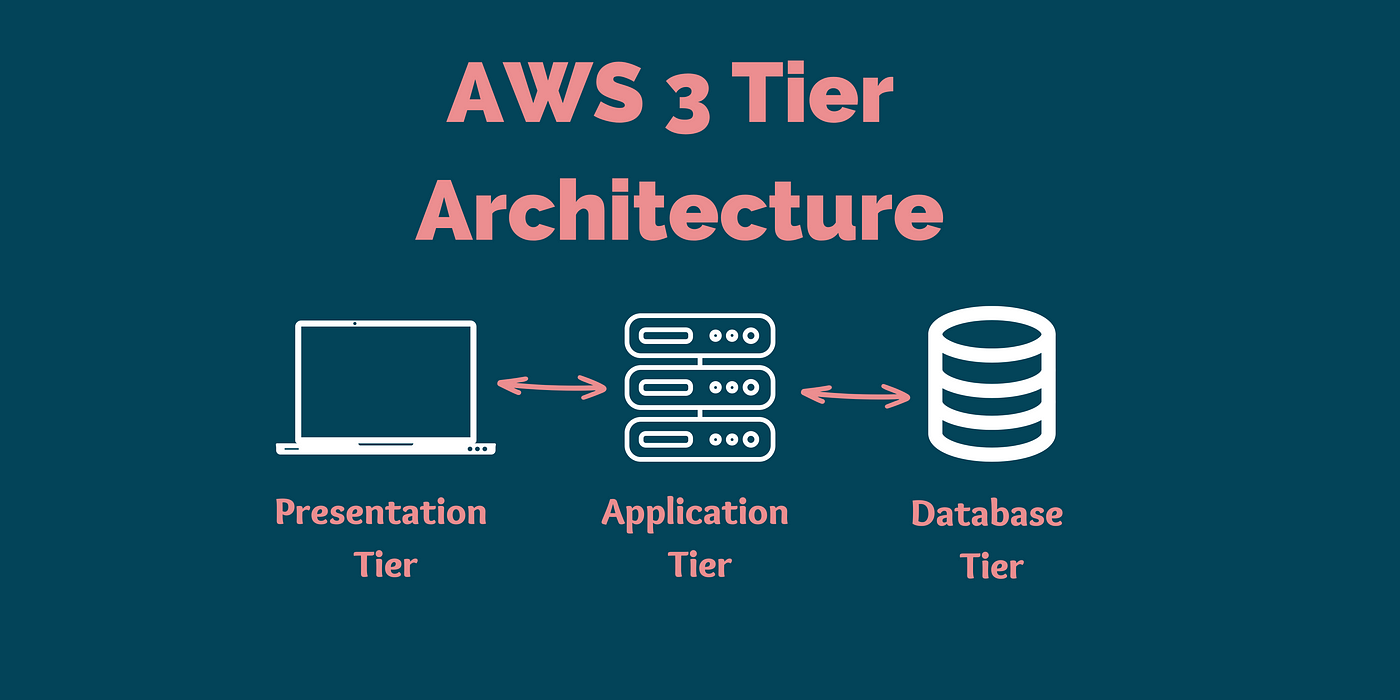
\includegraphics[width=100mm]{slike/arhitektura.png}
		\caption{Arhitektura sustava}
		\label{fig:arhitektura}
	\end{figure}

	\indent{\textit{\underline{Web preglednik}} je program koji korisniku omogućuje pregled
	web-stranica i multimedijalnih sadržaja vezanih uz njih. Svaki web preglednik je predvoditelj korištenja web aplikacija,
	jer omogućuje korisniku da preko web preglednika šalje zahtjeve web poslužitelju.}

	\indent{\textit{\underline{Web poslužitelj}} je osnova rada web aplikacije. On pokreće cijeli sustav rada aplikacije
	te joj prosljeđuje zahtjeve od korisnika. Osnovna zadaća web poslužitelja je omogućiti komunikaciju između korisnika i aplikacije, a ta
	komunikacija se odvija preko HTTP protokola. To je vrsta protokola koja se koristi za prijenos informacija na internetu.}

	\indent{\textit{\underline{Web aplikacija}} je dio web poslužitelja koja služi korisniku za obradu željenih zahtjeva.
	Web aplikacija radi tako da prima zahtjeve i ovisno o zahtjevu pristupa {\textit{\underline{bazi podataka}}} iz koje dohvaća
	"odgovore" na željene zahtjeve. Te "odgovore" šalje natrag korisniku preko web poslužitelja u obliku HTML dokumenta kojeg
	korisnik vidi u web pregledniku.}

	\indent{Programski jezik kojeg smo odabrali za izradu naše web aplikacije je Python. U sklopu Pythona koristimo Django, radni okvir koji služi za izradu web aplikacija. Razvojno okruženje koje koristimo
	je Microsoft Visual Studio Code. Arhitektura sustava temelji se na MVC odnosno MTV konceptu.}

	\indent{Django je modeliran oko MVC arhitekture, no svoju arhitekturu definira kao MTV (eng. {\textit{Model-Template-View}})
	arhitekturu. Komponentu upravitelj (eng. {\textit{Controller}}) zamjenjuje komponentom pogled (eng. {\textit{View}}) te
	komponentu pogled s komponentom predložak (eng. {\textit{Template}}). MTV razdvaja različite dijelove web-stranice: prikaz,
	pristup podatcima i logiku web stranice. Također omogućava neovisnu izgradnju web-stranica, povećava sigurnost sustava te
	pojednostavljuje održavanje sustava.}

	\noindent{MTV se sastoji od:}
	\begin{itemize}
		\item 	\textbf{Model} - definira oblike i odnose podataka u bazi podataka. Model u Django okruženju je klasa napisana
				u programskom jeziku Python. Određuje varijable i metode pridužene određenim tipovima podataka te ima značenje
				tablice u bazi podataka. Model je usko povezan s bazom podataka i pogledom. Od baze podataka model dohvaća tražene
				podatke i prosljeđuje ih pogledu.
		\item 	\textbf{Predložak} - sloj arhitekture MTV-a usko povezan s web-preglednikom. Predložak je HTML stranica s dodanim
				strukturama koje omogućavaju prikaz podataka koji su proslijeđeni od pogleda. Zadaća predloška je sadržaj primljen
				od pogleda organizirati i ugraditi u HTML kod koji će se prikazati u web-pregledniku.
		\item 	\textbf{Pogled} - određuje koji će podatci biti prikazani, odnosno, koji će podatci biti dohvaćeni iz baze podataka
				i prikazani pomoću predloška u web-pregledniku. U Djangu prilikom stvaranja nove web-aplikacije za svaku pojedinu
				aplikaciju stvara se zasebna datoteka pogleda. Pogled ne zna kako su podatci prikazani u web-pregledniku. Posao
				pogleda je dohvatiti tražene podatke i proslijediti ih višem sloju koji će ih prikazati u pregledniku.
	\end{itemize}
	
		

		

				
		\section{Baza podataka}
			
		{Potrebe sustava za bazu podataka su relativno jednostavne, a relacije između entiteta nisu osobito kompleksne. Zbog tih razloga, sustav za bazu podataka koristi MongoDB – \textit{NoSQL}, dokumentno-orijentiranu bazu podataka.} \\ {Entiteti za pohranjivanje podataka su:}
		\begin{itemize}
			\item 	\textbf{Word}{,}
			\item 	\textbf{PronunciationAudio}{,}
			\item 	\textbf{Dictionary}{,}
			\item 	\textbf{Account}{.}
			\item 	\textbf{WordProgress}{,}
			\item 	\textbf{DictionaryProgress}{.}
		\end{itemize}
		{Zvučni zapis izgovora riječi odvojen je od same riječi na koju se odnosi jer je zvučna datoteka relativno veća od ostatka podataka za riječ čime se ubrzava vrijeme dohvata riječi kada se ne koristi način učenja slovkanjem riječi uz dani izgovor.}
		
			\subsection{Opis tablica}
			

				\textit{Važno je istaknuti da je svakom MongoDB dokumentu automatski pridodjeljen , uz ostale atribute, jedinstveni ObjectId u "\_id" atributu (primarni ključ) te je on u tablicama prikazan samo ondje gdje se eksplicitno koristi.} \\
				
				\textbf{Word} \\ {Opisuje riječ. Više rječnika može sadržavati iste riječi pa je veza \textit{N..N}. Sadrži strani ključ na zvučni zapis izgovora riječi na ciljanom jeziku. Veza sa zvučnim zapisom je \textit{N..1}. Svi dokumenti entiteta \textbf{Word} sadržani su u kolekciji "Words".}
				
				\begin{longtblr}[
					label=none,
					entry=none
					]{
						width = \textwidth,
						colspec={|X[8,l]|X[6, l]|X[20, l]|}, 
						rowhead = 1,
					} %definicija širine tablice, širine stupaca, poravnanje i broja redaka naslova tablice
					\hline \SetCell[c=3]{c}{\textbf{Word}}	 \\ \hline[3pt]
					\SetCell{LightGreen}\_id & objectId	&  	Primarni ključ riječi.  	\\ \hline
					word & string	&  	Zapis riječi na ciljanom jeziku.  	\\ \hline
					translation	& string &   Prevedeni zapis riječi na hrvatskom.	\\ \hline 
					descriptionLang & string	&  	Opis riječi na ciljanom jeziku.	\\ \hline
					descriptionCro & string	&  	Opis riječi na hrvatskome jeziku.	\\ \hline  
					\SetCell{LightBlue} audio\_id	& objectId &   Primarni ključ zvučnog zapisa izgovora riječi na ciljanom jeziku.	\\ \hline 
				\end{longtblr}
				
				\textbf{PronunciationAudio} \\ {Sadrži zvučni zapis izgovora na ciljanom jeziku nekih riječi. Veza s riječima je \textit{1..N} u slučaju postojanja homofona. Svi dokumenti entiteta \textbf{PronunciationAudio} sadržani su u kolekciji "PronunciationAudios".}
				
				\begin{longtblr}[
					label=none,
					entry=none
					]{
						width = \textwidth,
						colspec={|X[8,l]|X[6, l]|X[20, l]|}, 
						rowhead = 1,
					} %definicija širine tablice, širine stupaca, poravnanje i broja redaka naslova tablice
					\hline \SetCell[c=3]{c}{\textbf{PronunciationAudio}}	 \\ \hline[3pt]
					\SetCell{LightGreen}\_id & objectId	&  	Primarni ključ zvučnog zapisa.  	\\ \hline
					audio	& binData &   Binarni zapis .mp3 datoteke zvučnog zapisa izgovora na ciljanom jeziku.	\\ \hline 
				\end{longtblr}
				
				\textbf{Dictionary} \\ {Opis rječnika. Riječi riječnika zapisane su kao polje referenci na dokumente entitete \textbf{word} u atributu "words". Veza s riječima je \textit{N..N} jer više rječnika mogu sadržavati istu riječ. Svi dokumenti entiteta \textbf{Dictionary} sadržani su u kolekciji "Dictionaries".}
				
				\begin{longtblr}[
					label=none,
					entry=none
					]{
						width = \textwidth,
						colspec={|X[8,l]|X[6, l]|X[20, l]|}, 
						rowhead = 1,
					} %definicija širine tablice, širine stupaca, poravnanje i broja redaka naslova tablice
					\hline \SetCell[c=3]{c}{\textbf{Dictionary}}	 \\ \hline[3pt]
					\SetCell{LightGreen}\_id & objectId	&  	Primarni ključ rječnika.  	\\ \hline
					name	& string &   Ime rječnika.	\\ \hline 
					language	& string &   Ciljani jezik rječnika.	\\ \hline
					\SetCell{LightBlue} words	& array &   Polje referenci na dokumenate riječi koje čine rječnik.	\\ \hline  
				\end{longtblr}
				
				\textbf{Account} \\ {Opis profila. Administratorske profile od učeničkih profila razlikujemo atributom "isAdmin". Svi dokumenti entiteta \textbf{Account} sadržani su u kolekciji "Accounts".}
				
				\begin{longtblr}[
					label=none,
					entry=none
					]{
						width = \textwidth,
						colspec={|X[8,l]|X[6, l]|X[20, l]|}, 
						rowhead = 1,
					} %definicija širine tablice, širine stupaca, poravnanje i broja redaka naslova tablice
					\hline \SetCell[c=3]{c}{\textbf{Account}}	 \\ \hline[3pt]
					\SetCell{LightGreen}\_id & objectId	&  	Primarni ključ profila.  	\\ \hline
					username	& string &   Korisničko ime profila. (Alternativni primarni ključ)	\\ \hline 
					email	& string &   Adresa e-pošte profila. (Alternativni primarni ključ)	\\ \hline 
					encryptedPass	& string &   SHA-256 kôd lozinke profila.	\\ \hline
					first\_name	& string &   Ime vlasnika profila.	\\ \hline 
					last\_name	& string &   Prezime vlasnika profila.	\\ \hline 
					isAdmin	& boolean &   Naznaka posjeduje li profil administratorske privilegije.	\\ \hline
					hasInitialPass	& boolean &   Naznaka je li korisnik promijenio inicijalnu lozinku dodijeljenju prilikom registracije. False ... inicijalna lozinka nije promijenjena.     True ... inicijalna lozinka je promijenjena.	\\ \hline  
				\end{longtblr}
				
				\textbf{WordProgress} \\ {Opis napretka učenja određene riječi. Dokumenti entiteta \textbf{WordProgress} pojavljuje se kao ugradbeni dokumenti u dokumentima entiteta \textbf{WordProgress}.}
				
				\begin{longtblr}[
					label=none,
					entry=none
					]{
						width = \textwidth,
						colspec={|X[8,l]|X[6, l]|X[20, l]|}, 
						rowhead = 1,
					} %definicija širine tablice, širine stupaca, poravnanje i broja redaka naslova tablice
					\hline \SetCell[c=3]{c}{\textbf{WordProgress}}	 \\ \hline[3pt]
					\SetCell{LightBlue} word\_id	& objectId &   Referenca na riječ čiji se napredak zabilježava.	\\ \hline 
					timeExpiry	& timestamp &   UNIX vrijeme nakon kojeg je riječ potrebno ponovno ispitati. Vrijeme posljednjeg ispitivanja + vrijeme isteka trenutne posude.	\\ \hline
					currBox	& int &   Trenutna posuda u kojoj se riječ nalazi. Dopuštene vrijednosti: 1, ..., n, n + 1. Ako se riječ nalazi u n + 1. posudi, smatra se naučenom.	\\ \hline
				\end{longtblr}
				
				\textbf{DictionaryProgress} \\ {Opis napretka učenja određenog rječnika od strane određenog učenika.  Svi dokumenti entiteta \textbf{DictionaryProgress} sadržani su u kolekciji "DictionariesProgress".}
				
				\begin{longtblr}[
					label=none,
					entry=none
					]{
						width = \textwidth,
						colspec={|X[8,l]|X[6, l]|X[20, l]|}, 
						rowhead = 1,
					} %definicija širine tablice, širine stupaca, poravnanje i broja redaka naslova tablice
					\hline \SetCell[c=3]{c}{\textbf{DictionaryProgress}}	 \\ \hline[3pt]
					\SetCell{LightBlue} account\_id	& objectId &   Referenca na profil koji uči referencirani rječnik.	\\ \hline 
					\SetCell{LightBlue} dict\_id	& objectId &   Referenca na rječnik kojeg referencirani profil aktivno uči.	\\ \hline
					learningMode	& int &   Trenutni način učenja referenciranog rječnika za referenciranog korisnika. Dopuštene vrijednosti: 1 (prijevod na ciljani jezik), 2 (prijevod na hrvatski), 3 (slovkanje), 4 (izgovor).	\\ \hline
					\SetCell{LightBlue} wordsProgress	& array &   Polje napretka svih riječi referenciranog rječnika, tj. polje ugrađenih dokumenata entiteta \textbf{WordProgress}.	\\ \hline 
				\end{longtblr}
			
			\subsection{Dijagram baze podataka}
			
			\textit{Važno je istaknuti da je svakom MongoDB dokumentu automatski pridodjeljen , uz ostale atribute, jedinstveni ObjectId u "\_id" atributu (primarni ključ) te je on u tablicama prikazan samo ondje gdje se eksplicitno koristi.} \\
				
			\begin{figure}[H]
				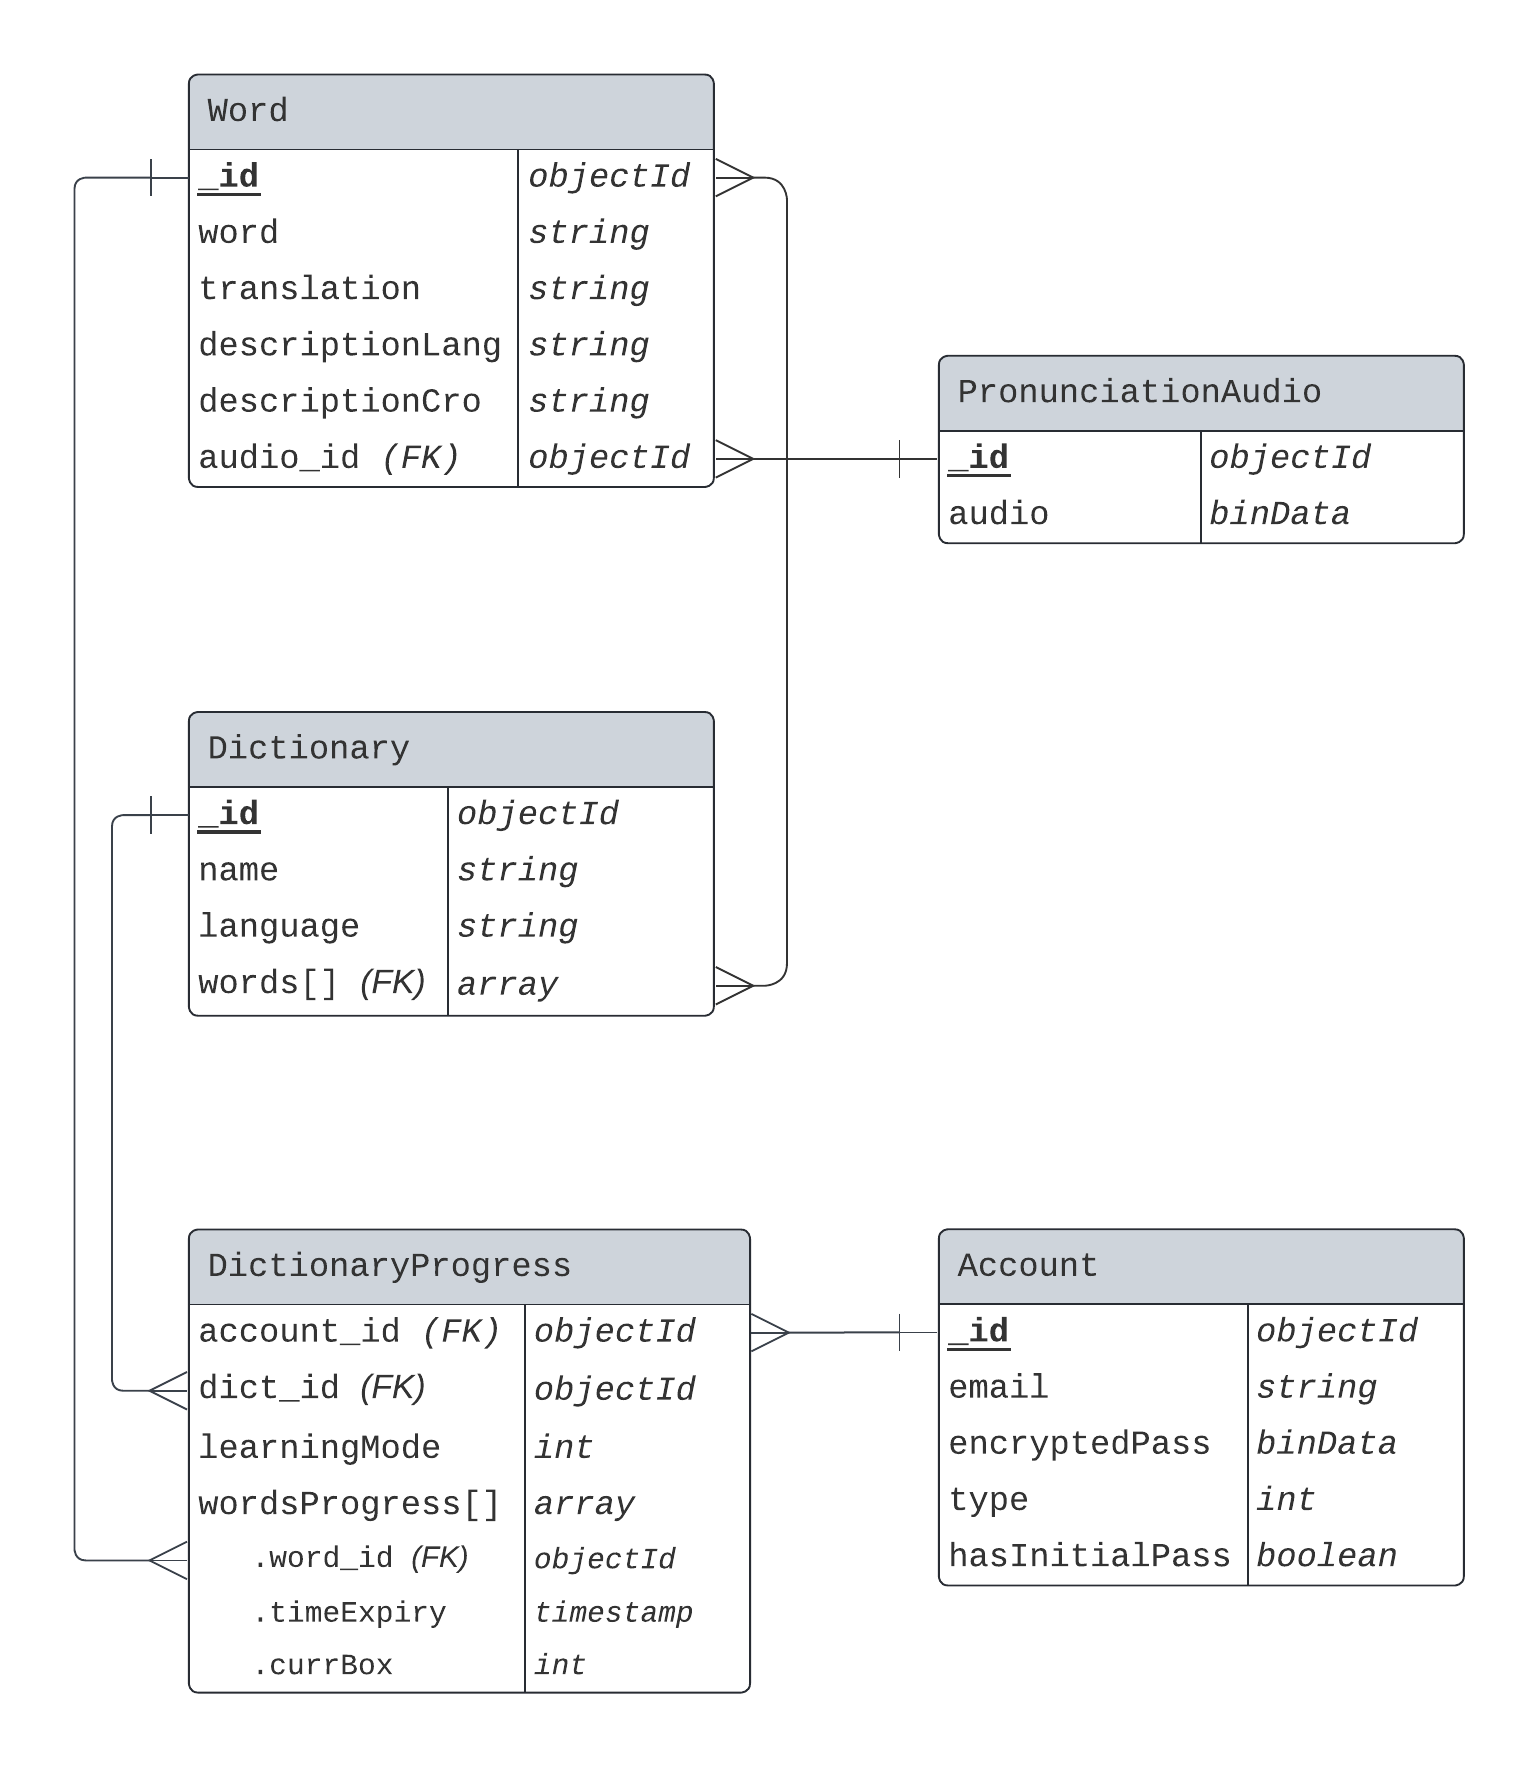
\includegraphics[width=\textwidth]{dijagrami/CanonPrinterDB_ER.png} %veličina u odnosu na širinu linije
				\caption{ER dijagram baze podataka}
				\label{fig:ER_dijagram} %label mora biti drugaciji za svaku sliku
			\end{figure}
			
			\eject
			
			
		\section{Dijagram razreda}

			\begin{figure}[H]
				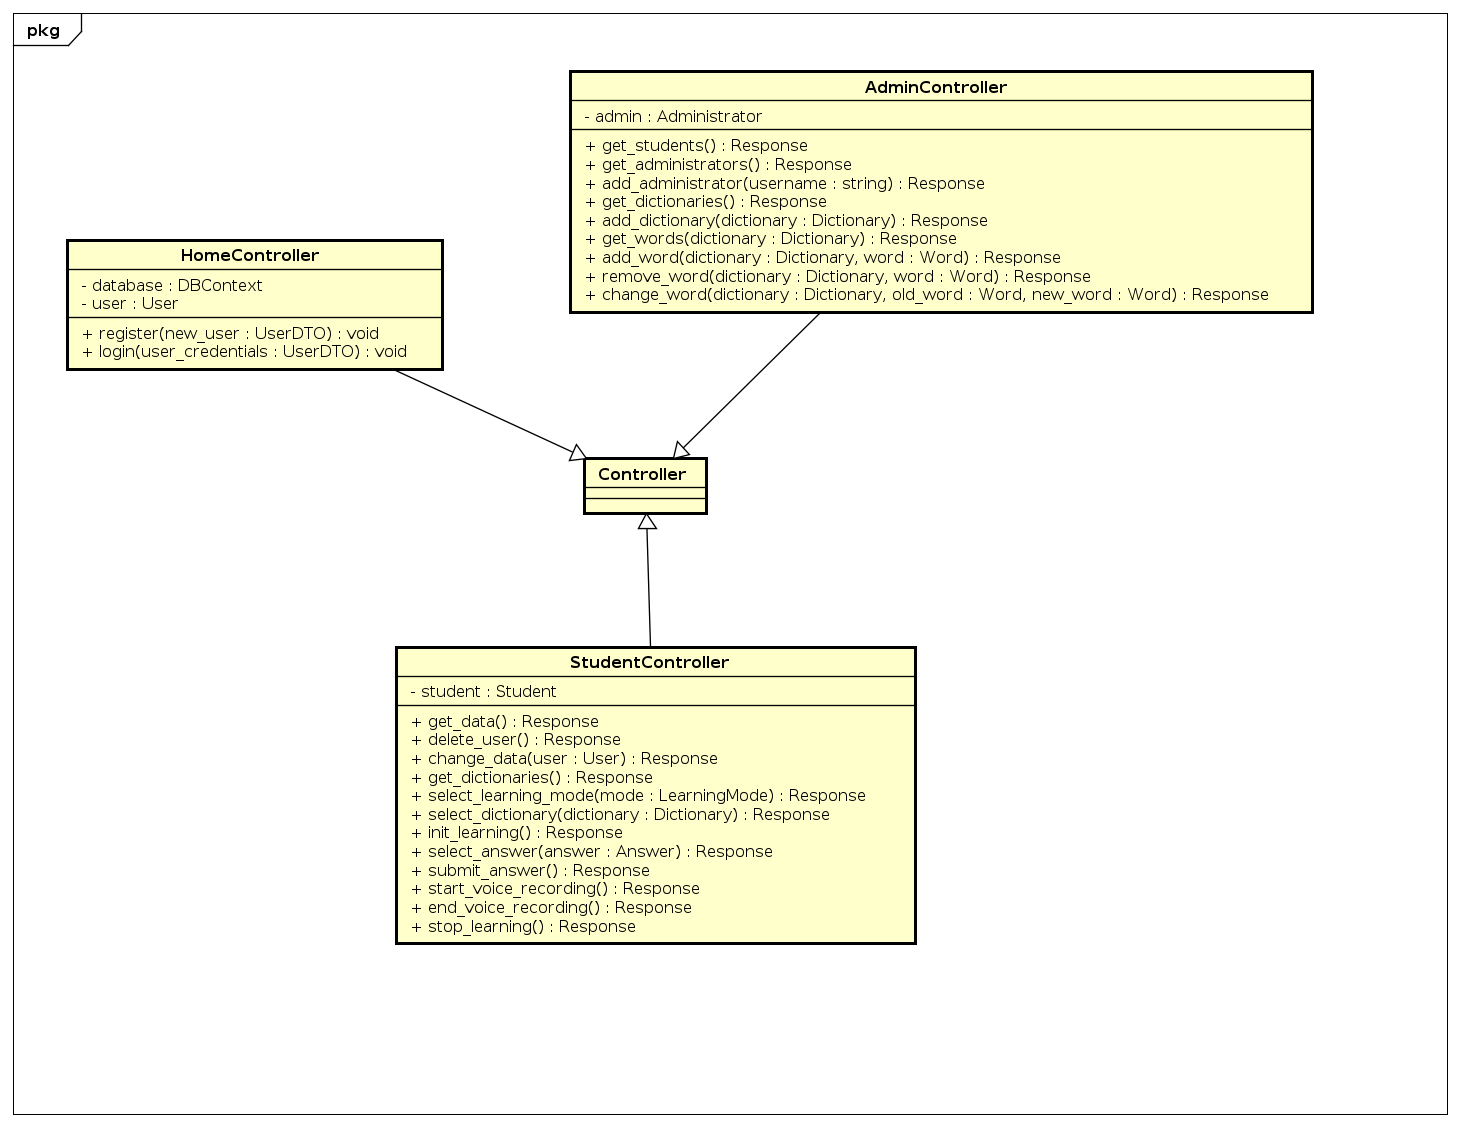
\includegraphics[width=\textwidth]{dijagrami/classcont.png} %veličina u odnosu na širinu linije
				\caption{Dijagram razreda - dio Controllers}
				\label{fig:classcont} %label mora biti drugaciji za svaku sliku
			\end{figure}

			\begin{figure}[H]
				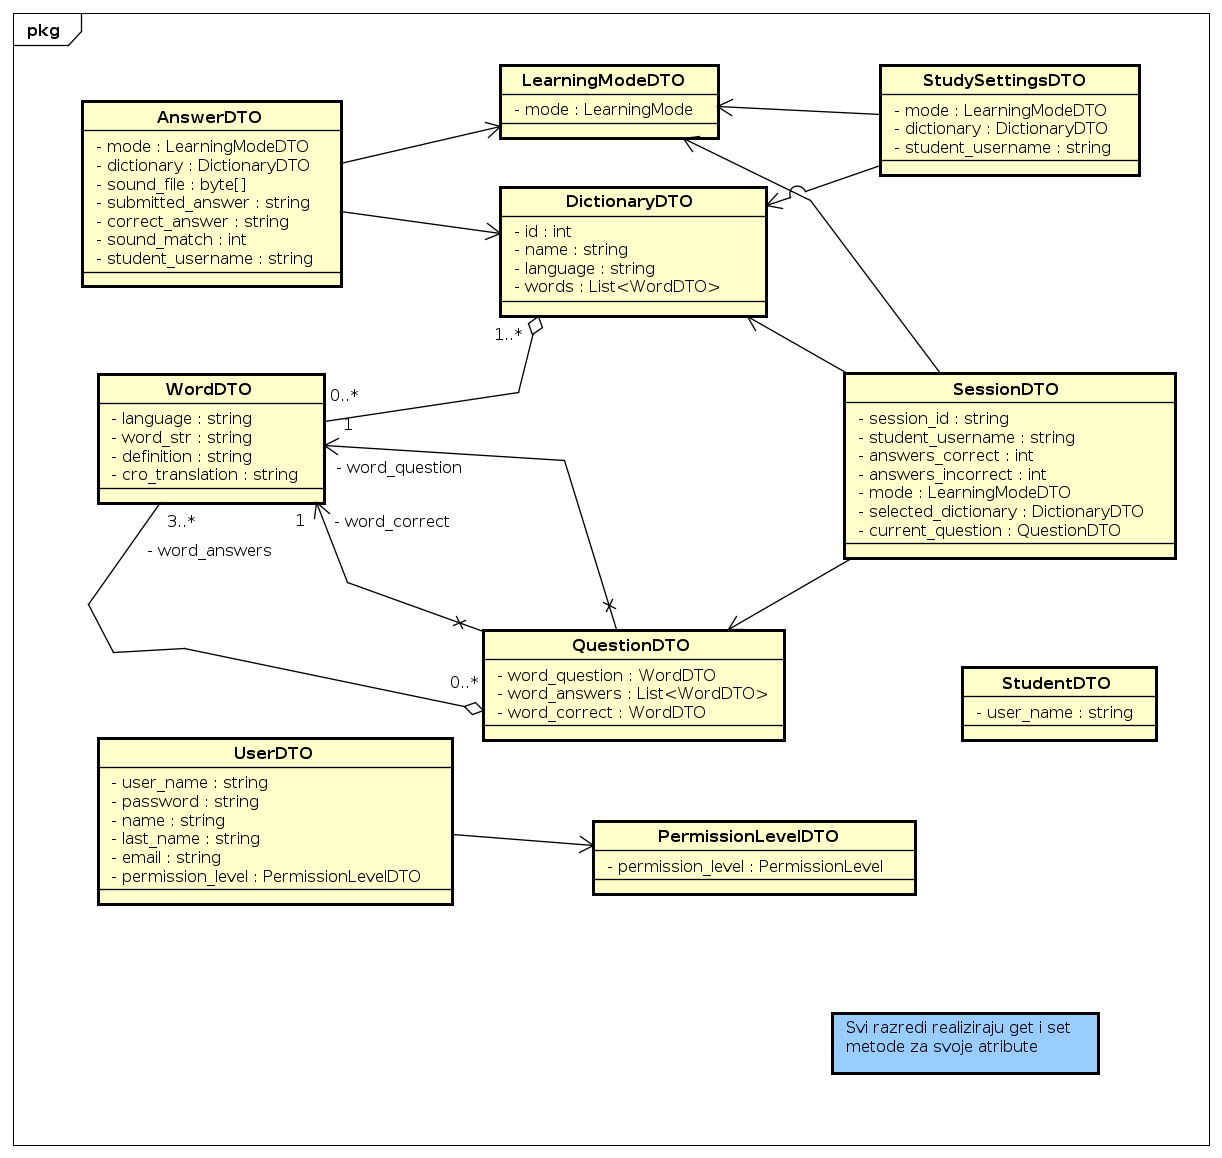
\includegraphics[width=\textwidth]{dijagrami/classdto.png} %veličina u odnosu na širinu linije
				\caption{Dijagram razreda - dio Data Transfer Objects}
				\label{fig:classdto} %label mora biti drugaciji za svaku sliku
			\end{figure}

			\begin{figure}[H]
				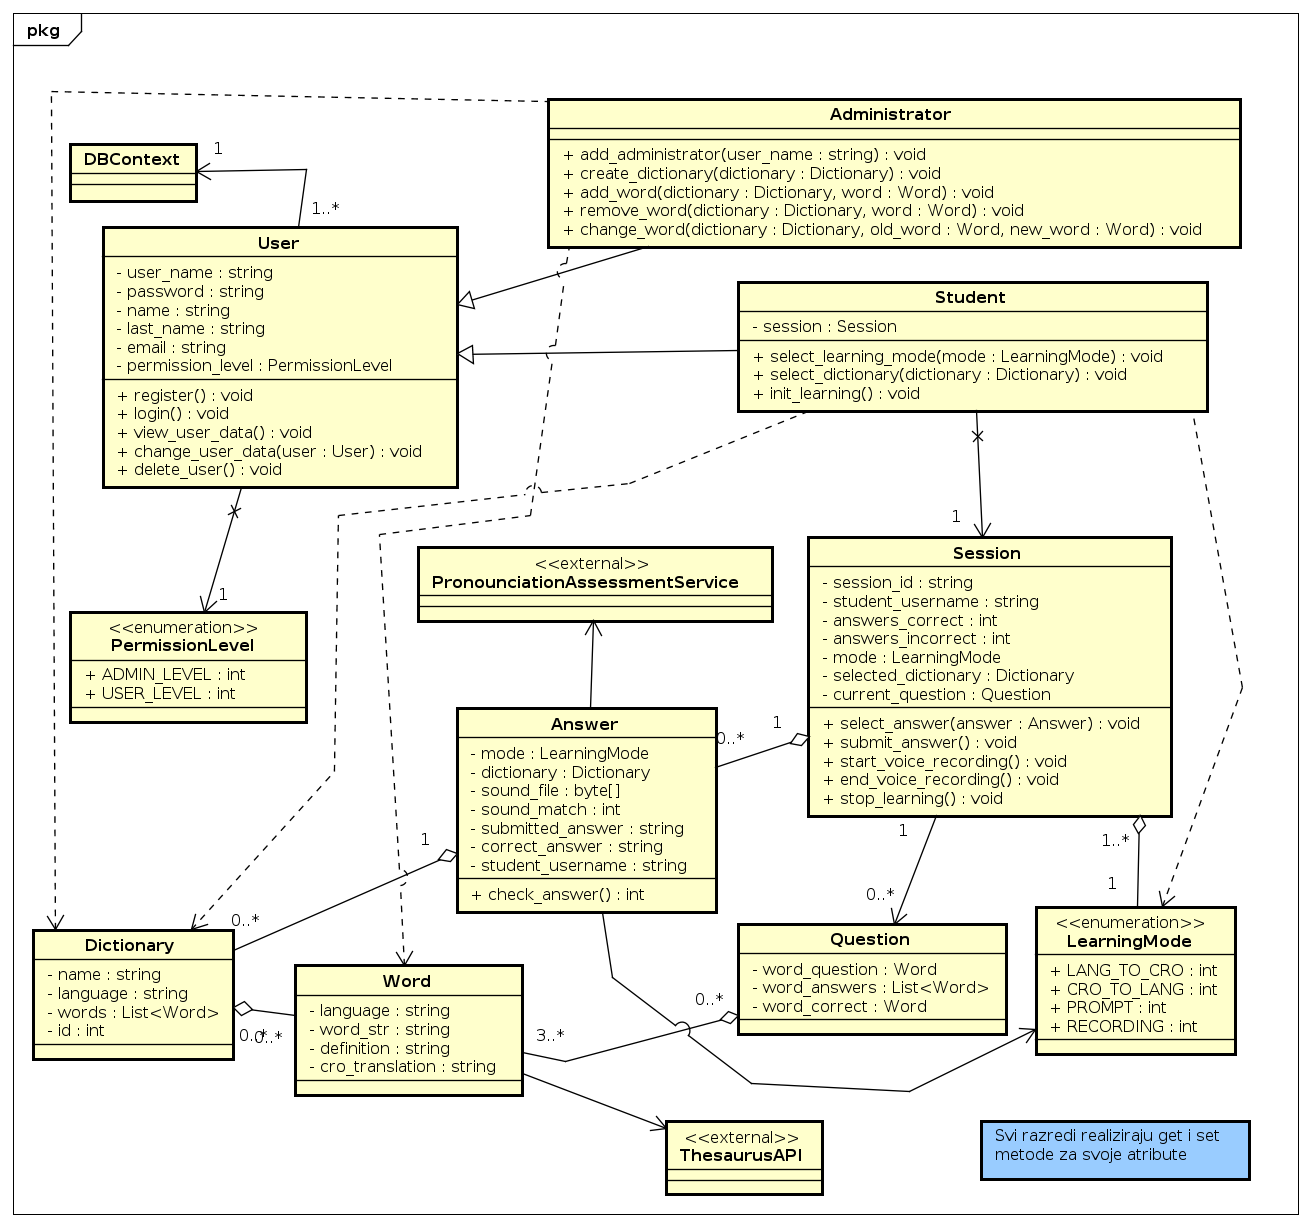
\includegraphics[width=\textwidth]{dijagrami/classmodel.png} %veličina u odnosu na širinu linije
				\caption{Dijagram razreda - dio Models}
				\label{fig:classmodel} %label mora biti drugaciji za svaku sliku
			\end{figure}
		
			\textit{Potrebno je priložiti dijagram razreda s pripadajućim opisom. Zbog preglednosti je moguće dijagram razlomiti na više njih, ali moraju biti grupirani prema sličnim razinama apstrakcije i srodnim funkcionalnostima.}\\
			
			\textbf{\textit{dio 1. revizije}}\\
			
			\textit{Prilikom prve predaje projekta, potrebno je priložiti potpuno razrađen dijagram razreda vezan uz \textbf{generičku funkcionalnost} sustava. Ostale funkcionalnosti trebaju biti idejno razrađene u dijagramu sa sljedećim komponentama: nazivi razreda, nazivi metoda i vrste pristupa metodama (npr. javni, zaštićeni), nazivi atributa razreda, veze i odnosi između razreda.}\\
			
			\textbf{\textit{dio 2. revizije}}\\			
			
			\textit{Prilikom druge predaje projekta dijagram razreda i opisi moraju odgovarati stvarnom stanju implementacije}
			
			
			
			\eject
		
		\section{Dijagram stanja}
			
			
			\textbf{\textit{dio 2. revizije}}\\
			
			\textit{Potrebno je priložiti dijagram stanja i opisati ga. Dovoljan je jedan dijagram stanja koji prikazuje \textbf{značajan dio funkcionalnosti} sustava. Na primjer, stanja korisničkog sučelja i tijek korištenja neke ključne funkcionalnosti jesu značajan dio sustava, a registracija i prijava nisu. }
			
			
			\eject 
		
		\section{Dijagram aktivnosti}
			
			\textbf{\textit{dio 2. revizije}}\\
			
			 \textit{Potrebno je priložiti dijagram aktivnosti s pripadajućim opisom. Dijagram aktivnosti treba prikazivati značajan dio sustava.}
			
			\eject
		\section{Dijagram komponenti}
		
			\textbf{\textit{dio 2. revizije}}\\
		
			 \textit{Potrebno je priložiti dijagram komponenti s pripadajućim opisom. Dijagram komponenti treba prikazivati strukturu cijele aplikacije.}